\usetikzlibrary{3d}
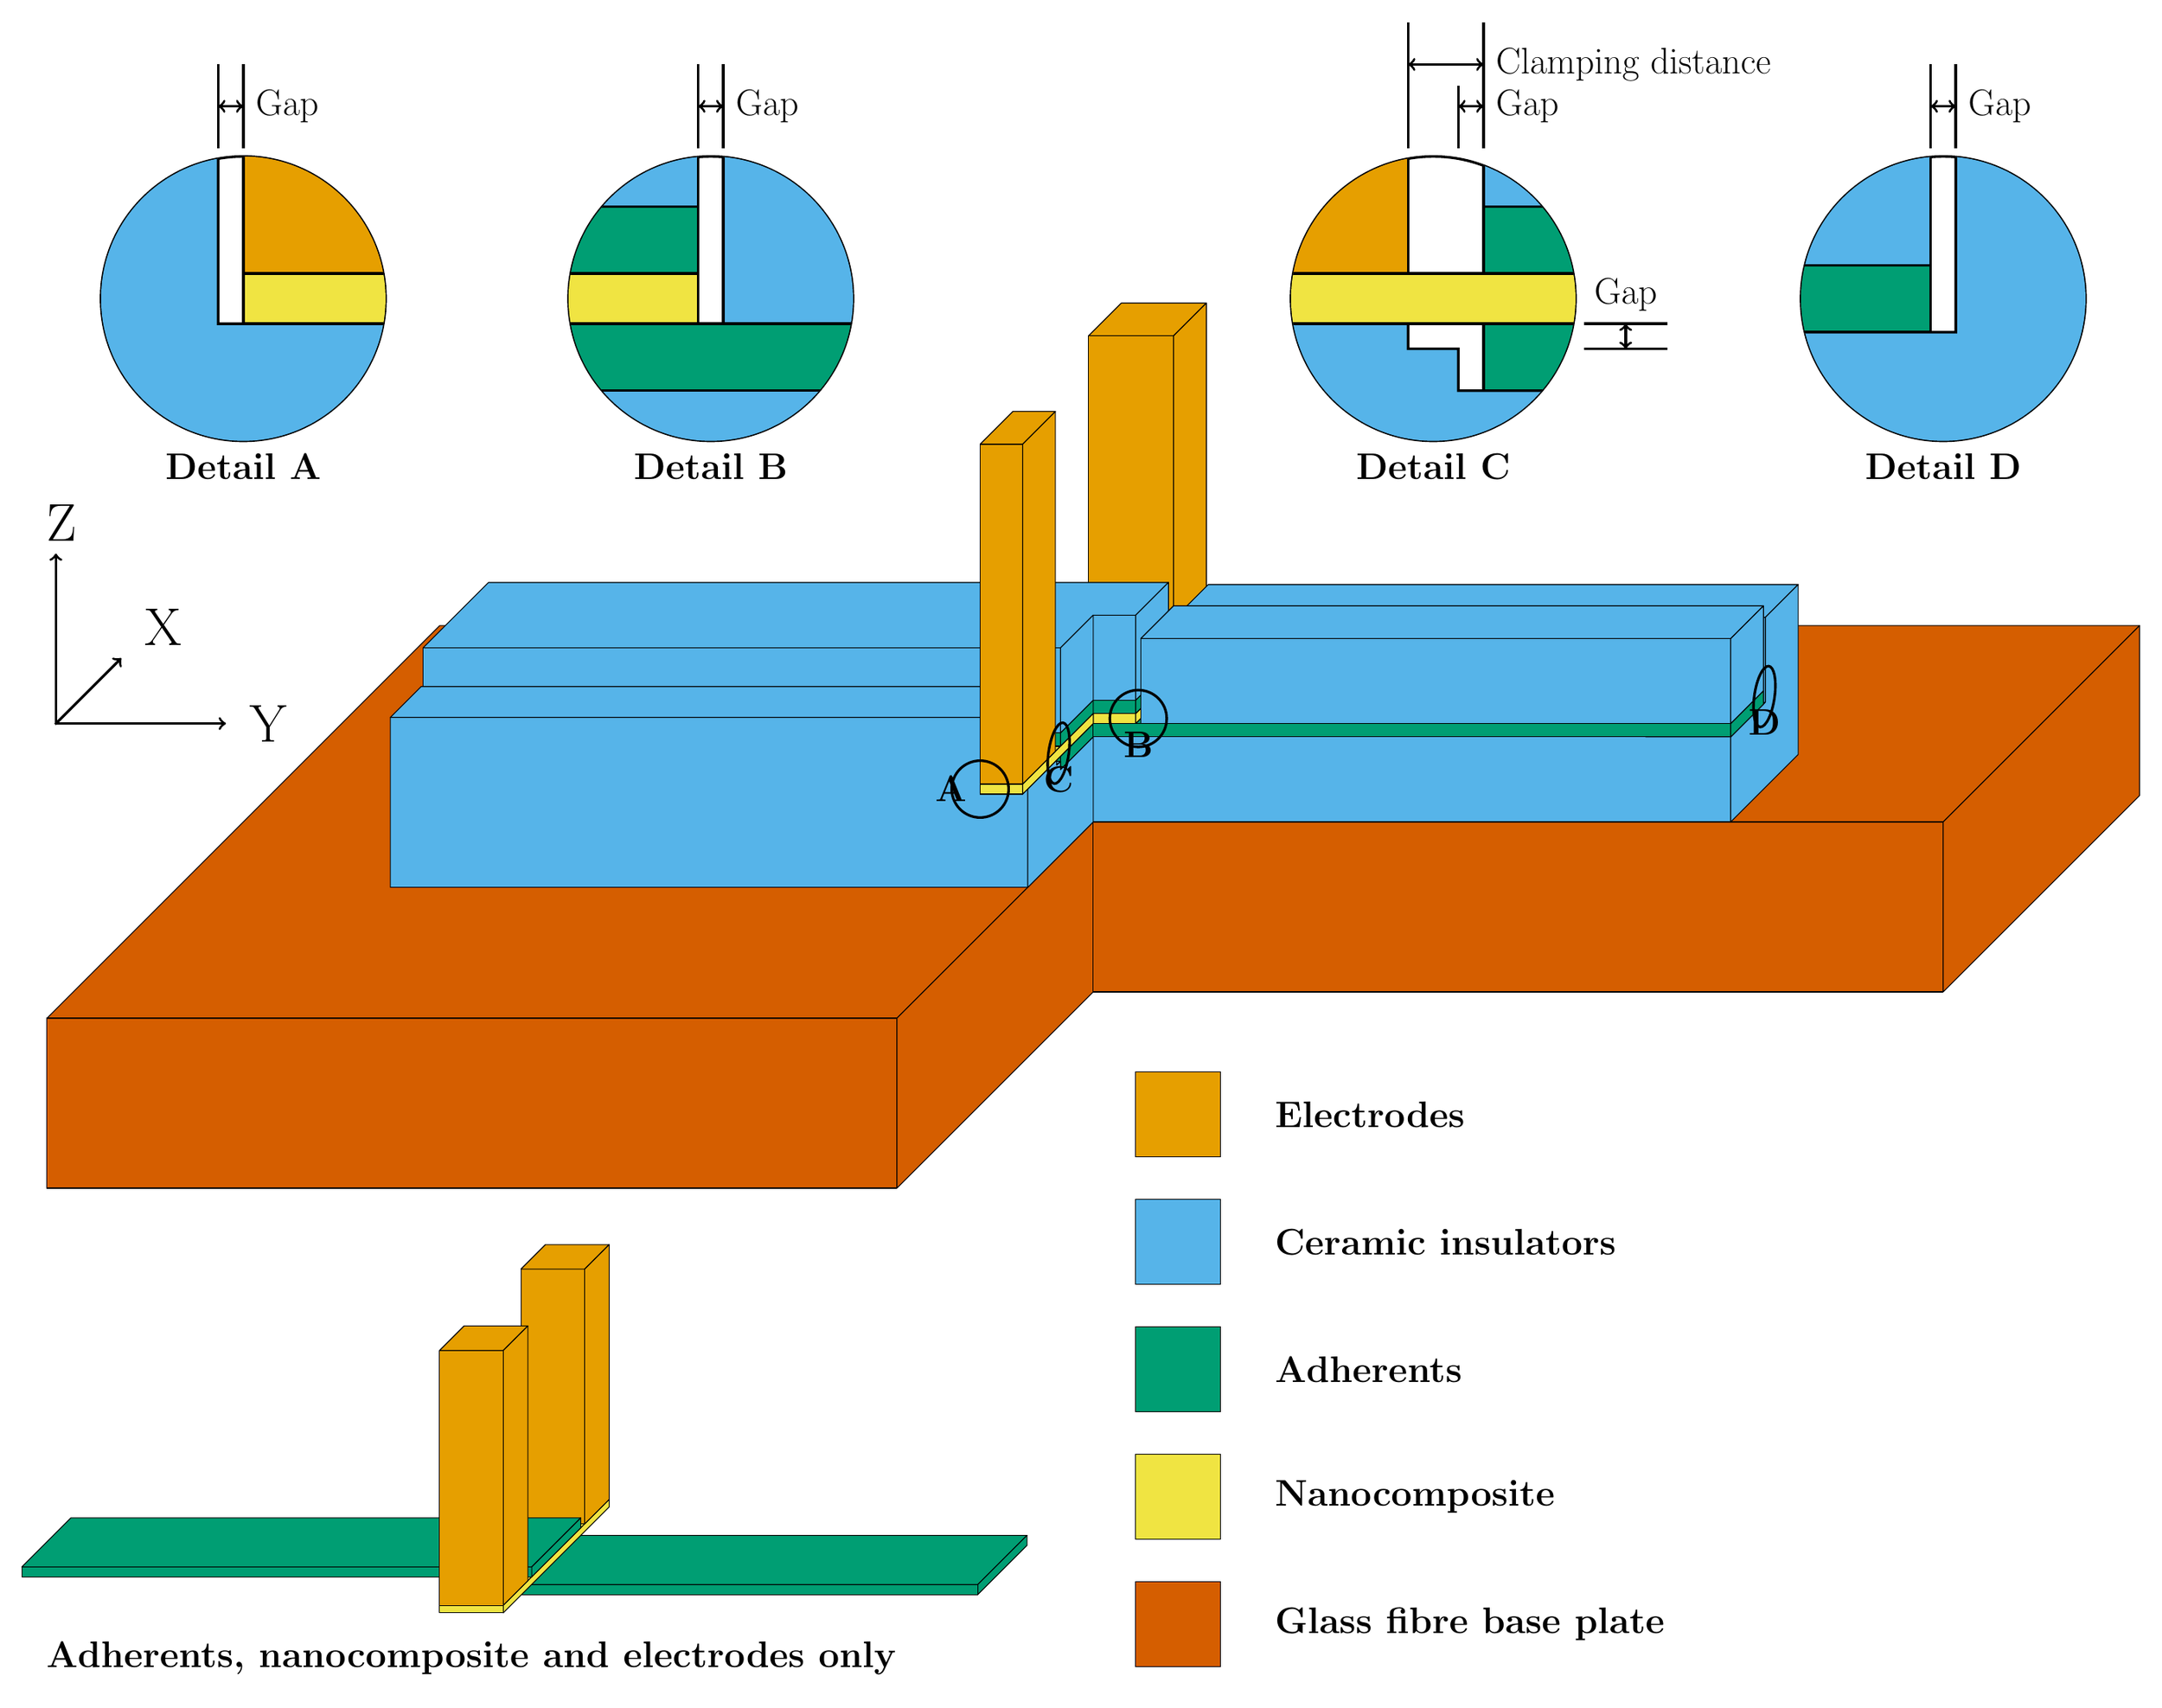
\begin{tikzpicture}[scale=0.11]
\LARGE

%Overlap distance
\def \overlap{12.7}

%Clamping distance
\def \cdistance{1.5}

%Thermal discontinuities gap
\def \gap{0.75}

%Electrodes dimensions
\def \telectrode{0.5*25.4}
\def \helectrode{2*25.4}

%Dimensions des adhérent
\def \ladherent{4*25.4}
\def \tadherent{2.0}
\def \wadherent{25.4}

%Nanocomposite dimensions
\def \tnano{1.5}
\def \lnano{54.8}
\def \wnano{\overlap}

%Ceramic insulators
\def \tceramic{0.5*25.4}
\def \hceramic{25.4}

%Composite base plate
\def \tcompositeplate{25.4}
\def \lcompositeplate{10*25.4}
\def \wcompositeplate{6*25.4}

%Position et taille des annotations
\def \dia{4.25}
\def \detailscale{5}
\def \legend{12.7}
\def \distcotation{2.5}

%Colour palette for colourbliness
\definecolor{orange}{rgb}{0.902,0.624,0}
\definecolor{skyblue}{rgb}{0.337,0.7058,0.9137}
\definecolor{bluegreen}{rgb}{0,0.6196,0.4509}
\definecolor{yellow}{rgb}{0.9411,0.8941,0.2588}
\definecolor{blue}{rgb}{0,0.4471,0.6980}
\definecolor{vermillion}{rgb}{0.8353,0.3686,0}
\definecolor{purple}{rgb}{0.8,0.4745,0.6549}

\def \colelectrode{orange}
\def \colceramic{skyblue}l
\def \coladherent{bluegreen}
\def \colnano{yellow}
\def \colbase{vermillion}

%GF composite base
\begin{scope}[,line join=round]
	\draw[black,fill=\colbase] (0,-\tadherent-\tceramic,0) -- ++(0,0,0.5*\wcompositeplate) -- ++(-0.5*\lcompositeplate,0,0) -- ++(0,0,-\wcompositeplate)  -- ++(\lcompositeplate,0,0)   -- ++(0,0,0.5*\wcompositeplate) -- cycle; %Top face
	\draw[black,fill=\colbase] (-0.5*\lcompositeplate,-\tadherent-\tceramic,0.5*\wcompositeplate) -- ++(0,-\tcompositeplate,0) -- ++(0.5*\lcompositeplate,0,0) -- ++(0,\tcompositeplate,0)  -- cycle; %Bottom left
	\draw[black,fill=\colbase] (0,-\tadherent-\tceramic,0.5*\wcompositeplate) -- ++(0,-\tcompositeplate,0) -- ++(0,0,-0.5*\wcompositeplate) -- ++(0,\tcompositeplate,0)  -- cycle; %Bottom middle left
	\draw[black,fill=\colbase] (0,-\tadherent-\tceramic,0) -- ++(0,-\tcompositeplate,0) -- ++(0.5*\lcompositeplate,0,0) -- ++(0,\tcompositeplate,0)  -- cycle; %Bottom middle right
	\draw[black,fill=\colbase] (0.5*\lcompositeplate,-\tadherent-\tceramic,0) -- ++(0,-\tcompositeplate,0) -- ++(0,0,-0.5*\wcompositeplate) -- ++(0,\tcompositeplate,0)  -- cycle; %Bottom right
\end{scope}

%Lower adherent
\begin{scope}[shift={(-0.5*\overlap,-\tadherent,0.5*\wadherent)},line join=round]
	\draw[black,fill=\coladherent] (0,0,0) -- ++(0.5*\overlap,0,0) --  ++(0,\tadherent,0)  -- ++(-0.5*\overlap,0,0)  -- cycle; % Front 1
	\draw[black,fill=\coladherent] (0.5*\overlap,0,-0.5*\wadherent) -- ++(\ladherent-0.5*\overlap,0,0) --  ++(0,\tadherent,0)  -- ++(-\ladherent+0.5*\overlap,0,0)  -- cycle; % Front 2
	\draw[black,fill=\coladherent] (0,\tadherent,0) -- ++(0.5*\overlap,0,0) -- ++(0,0,-0.5*\wadherent) --++ (\ladherent-0.5*\overlap,0,0) -- ++(0,0,-0.5*\wadherent) -- ++(-\ladherent,0,0)  -- cycle; % Top
	\draw[black,fill=\coladherent] (0.5*\overlap,0,0) -- ++(0,\tadherent,0) -- ++(0,0,-0.5*\wadherent) -- ++(0,-\tadherent,0)  -- cycle; % Side 1
	\draw[black,fill=\coladherent] (\ladherent,0,-0.5*\wadherent) -- ++(0,\tadherent,0) -- ++(0,0,-0.5*\wadherent) -- ++(0,-\tadherent,0)  -- cycle; % Side 2
\end{scope}

%Nanocomposite
\begin{scope}[shift={(-0.5*\overlap,0,0.5*\lnano)},line join=round]
	\draw[black,fill=\colnano] (0,0,0) -- ++(0.5*\overlap,0,0) --  ++(0,\tnano,0)  -- ++(-0.5*\overlap,0,0)  -- cycle; % Front 1
	\draw[black,fill=\colnano] (0.5*\overlap,0,-0.5*\lnano) -- ++(0.5*\overlap,0,0) --  ++(0,\tnano,0)  -- ++(-0.5*\overlap,0,0)  -- cycle; % Front 2
	\draw[black,fill=\colnano] (0,\tnano,0) -- ++(0.5*\overlap,0,0) -- ++(0,0,-0.5*\lnano) --++ (0.5*\overlap,0,0) -- ++(0,0,-0.5*\lnano) -- ++(-\overlap,0,0)  -- cycle; % Top
	\draw[black,fill=\colnano] (0.5*\overlap,0,0) -- ++(0,\tnano,0) -- ++(0,0,-0.5*\lnano) -- ++(0,-\tnano,0)  -- cycle; % Side 1
	\draw[black,fill=\colnano] (\overlap,0,-0.5*\lnano) -- ++(0,\tnano,0) -- ++(0,0,-0.5*\lnano) -- ++(0,-\tnano,0)  -- cycle; % Side 2
\end{scope}

%Back electrode
\begin{scope}[shift={(-0.5*\overlap,\tnano,-0.5*\lnano+\telectrode)},line join=round]
	\draw[black,fill=\colelectrode] (0,0,0) -- ++(\overlap,0,0) --  ++(0,\helectrode,0)  -- ++(-\overlap,0,0)  -- cycle; % Front
	\draw[black,fill=\colelectrode] (0,\helectrode,0) -- ++(\overlap,0,0) -- ++(0,0,-\telectrode) -- ++(-\overlap,0,0)  -- cycle; % Top
	\draw[black,fill=\colelectrode] (\overlap,0,0) -- ++(0,\helectrode,0) -- ++(0,0,-\telectrode) -- ++(0,-\helectrode,0)  -- cycle; % Side
\end{scope}

%Upper adherent
\begin{scope}[shift={(-\ladherent+0.5*\overlap,\tnano,0.5*\wadherent)},line join=round]
\draw[black,fill=\coladherent] (0,0,0) -- ++(\ladherent-0.5*\overlap,0,0) --  ++(0,\tadherent,0)  -- ++(-\ladherent+0.5*\overlap,0,0)  -- cycle; % Front 1
	\draw[black,fill=\coladherent] (\ladherent-0.5*\overlap,0,-0.5*\wadherent) -- ++(0.5*\overlap,0,0) --  ++(0,\tadherent,0)  -- ++(-0.5*\overlap,0,0)  -- cycle; % Front 2
	\draw[black,fill=\coladherent] (0,\tadherent,0) -- ++(\ladherent-0.5*\overlap,0,0) -- ++(0,0,-0.5*\wadherent) --++ (0.5*\overlap,0,0) -- ++(0,0,-0.5*\wadherent) -- ++(-\ladherent,0,0)  -- cycle; % Top
	\draw[black,fill=\coladherent] (\ladherent-0.5*\overlap,0,0) -- ++(0,\tadherent,0) -- ++(0,0,-0.5*\wadherent) -- ++(0,-\tadherent,0)  -- cycle; % Side 1
	\draw[black,fill=\coladherent] (\ladherent,0,-0.5*\wadherent) -- ++(0,\tadherent,0) -- ++(0,0,-0.5*\wadherent) -- ++(0,-\tadherent,0)  -- cycle; % Side 2
\end{scope}

%Upper ceramic 1
\begin{scope}[shift={(-\ladherent+0.5*\overlap,\tnano+\tadherent,0.5*\wadherent)},line join=round]
\draw[black,fill=\colceramic] (0,0,0) -- ++(\ladherent-0.5*\overlap,0,0) --  ++(0,\tceramic,0)  -- ++(-\ladherent+0.5*\overlap,0,0)  -- cycle; % Front 1
	\draw[black,fill=\colceramic] (\ladherent-0.5*\overlap,0,-0.5*\wadherent) -- ++(0.5*\overlap,0,0) --  ++(0,\tceramic,0)  -- ++(-0.5*\overlap,0,0)  -- cycle; % Front 2
	\draw[black,fill=\colceramic] (0,\tceramic,0) -- ++(\ladherent-0.5*\overlap,0,0) -- ++(0,0,-0.5*\wadherent) --++ (0.5*\overlap,0,0) -- ++(0,0,-0.5*\wadherent) -- ++(-\ladherent,0,0)  -- cycle; % Top
	\draw[black,fill=\colceramic] (\ladherent-0.5*\overlap,0,0) -- ++(0,\tceramic,0) -- ++(0,0,-0.5*\wadherent) -- ++(0,-\tceramic,0)  -- cycle; % Side 1
	\draw[black,fill=\colceramic] (\ladherent,0,-0.5*\wadherent) -- ++(0,\tceramic,0) -- ++(0,0,-0.5*\wadherent) -- ++(0,-\tceramic,0)  -- cycle; % Side 2
\end{scope}

%Lower ceramic
\begin{scope}[shift={(-\ladherent+0.5*\overlap,-\tadherent-\tceramic,0.5*\wadherent+\tceramic)},line join=round]
	\draw[black,fill=\colceramic] (0,0,0) -- ++(\ladherent-0.5*\overlap,0,0) --  ++(0,\tceramic+\tadherent,0)  -- ++(-0.5*\overlap,0,0)  -- ++(0,\hceramic-\tceramic-\tadherent,0)  -- ++(-\ladherent+\overlap,0,0) -- cycle; % Front 1
	\draw[black,fill=\colceramic] (\ladherent-0.5*\overlap,0,-0.5*\wadherent-\tceramic) -- ++(\ladherent-0.5*\overlap,0,0) --  ++(0,\tceramic,0)  -- ++(-\ladherent+0.5*\overlap,0,0)  -- cycle; % Front 2
	\draw[black,fill=\colceramic] (2*\ladherent-\overlap,\tceramic,-\wadherent-\tceramic-\gap) -- ++(-\overlap,0,0) --  ++(0,\tceramic,0)  -- ++(\overlap,0,0)  -- cycle; % Front 3
	\draw[black,fill=\colceramic] (0,\hceramic,0) -- ++(\ladherent-\overlap,0,0) -- ++(0,0,-\tceramic+\gap) --++ (-\ladherent+\overlap,0,0) -- ++(0,0,\tceramic-\gap)  -- cycle; % Top
	\draw[black,fill=\colceramic] (2*\ladherent-\overlap,\tceramic,-0.5*\wadherent-\tceramic) -- ++(-\overlap,0,0) -- ++(0,0,-0.5*\wadherent-\gap) --++ (\overlap,0,0) -- ++(0,0,0.5*\wadherent+\gap)  -- cycle; % Top 2
	\draw[black,fill=\colceramic] (\ladherent+\gap,\hceramic,-\tceramic-\gap-\wadherent) -- ++(\ladherent-\overlap-\gap,0,0) -- ++(0,0,-\tceramic,0) --++ (-\ladherent+\overlap+\gap,0,0)  -- cycle; % Top 3
	\draw[black,fill=\colceramic] (\ladherent-\overlap,\tceramic+\tadherent-\gap,-\tceramic+\cdistance) -- ++(0.5*\overlap,0,0) -- ++(0,0,-\cdistance) --++ (-0.5*\overlap,0,0)  -- cycle; % Top 4 (gap)
	\draw[black,fill=\colceramic] (\ladherent-0.5*\overlap,0,0) -- ++(0,\tceramic+\tadherent,0) -- ++(0,0,-\tceramic+\cdistance) -- ++(0,-\gap,0) -- ++(0,0,-\cdistance) -- ++(0,-\tadherent+\gap,0) -- ++(0,0,-0.5*\wadherent) -- ++(0,-\tceramic,0)  -- cycle; % Side 1
	\draw[black,fill=\colceramic] (2*\ladherent-\overlap,0,-0.5*\wadherent-\tceramic) -- ++(0,\tceramic,0) -- ++(0,0,-0.5*\wadherent-\gap) -- ++(0,\hceramic-\tceramic,0) -- ++(0,0,-\tceramic) -- ++(0,-\hceramic,0) -- cycle; % Side 2
\end{scope}

%Lower adherent redraw
\begin{scope}[shift={(-0.5*\overlap,-\tadherent,0.5*\wadherent)},line join=round]
	\draw[black,fill=\coladherent] (0.5*\overlap,0,-0.5*\wadherent) -- ++(\ladherent-0.5*\overlap,0,0) --  ++(0,\tadherent,0)  -- ++(-\ladherent+0.5*\overlap,0,0)  -- cycle; % Front 2
	\draw[black,fill=\coladherent] (\ladherent,0,-0.5*\wadherent) -- ++(0,\tadherent,0) -- ++(0,0,-0.5*\wadherent) -- ++(0,-\tadherent,0)  -- cycle; % Side 2
\end{scope}

%Nanocomposite redraw
\begin{scope}[shift={(-0.5*\overlap,0,0.5*\lnano)},line join=round]
	\draw[black,fill=\colnano] (0,0,0) -- ++(0.5*\overlap,0,0) --  ++(0,\tnano,0)  -- ++(-0.5*\overlap,0,0)  -- cycle; % Front 1
	\draw[black,fill=\colnano] (0.5*\overlap,0,0) -- ++(0,\tnano,0) -- ++(0,0,-0.5*\lnano) -- ++(0,-\tnano,0)  -- cycle; % Side 1
\end{scope}

%Upper ceramic 2
\begin{scope}[shift={(0.5*\overlap+\gap,0,-00)},line join=round]
	\draw[black,fill=\colceramic] (0,0,0) -- ++(\ladherent-\overlap-\gap,0,0) --  ++(0,\tceramic,0)  -- ++(-\ladherent+\overlap+\gap,0,0)  -- cycle; % Front
	\draw[black,fill=\colceramic] (0,\tceramic,0) -- ++(\ladherent-\overlap-\gap,0,0) -- ++(0,0,-\telectrode) -- ++(-\ladherent+\overlap+\gap,0,0)  -- cycle; % Top
	\draw[black,fill=\colceramic] (\ladherent-\overlap-\gap,0,0) -- ++(0,\tceramic,0) -- ++(0,0,-\telectrode) -- ++(0,-\tceramic,0)  -- cycle; % Side
\end{scope}

%Front electrode
\begin{scope}[shift={(-0.5*\overlap,\tnano,0.5*\lnano)},line join=round]
	\draw[black,fill=\colelectrode] (0,0,0) -- ++(0.5*\overlap,0,0) --  ++(0,\helectrode,0)  -- ++(-0.5*\overlap,0,0)  -- cycle; % Front
	\draw[black,fill=\colelectrode] (0,\helectrode,0) -- ++(0.5*\overlap,0,0) -- ++(0,0,-\telectrode) -- ++(-0.5*\overlap,0,0)  -- cycle; % Top
	\draw[black,fill=\colelectrode] (0.5*\overlap,0,0) -- ++(0,\helectrode,0) -- ++(0,0,-\telectrode) -- ++(0,-\helectrode,0)  -- cycle; % Side
\end{scope}

%Circle for detail A
\begin{scope}[shift={(-0.5*\overlap,0.5*\tnano,0.5*\lnano)}]
	\draw[very thick, black] (0,0,0) circle[radius=\dia] node[left=0.1*\dia] {\textbf{\LARGE{A}}};
\end{scope}

%Circle for detail B
\begin{scope}[shift={(0.5*\overlap+0.5*\gap,0.5*\tnano,0)}]
	\draw[very thick, black] (0,0,0) circle[radius=\dia] node[below=0.1*\dia] {\textbf{\LARGE{B}}};
\end{scope}

%Circle for detail C
\begin{scope}[canvas is zy plane at x=0]
	\draw[very thick, black] (0.5*\wadherent+0.5*\cdistance,0.5*\tnano) circle[radius=\dia] node[below=0.1*\dia] {\textbf{\LARGE{C}}};
\end{scope}

%Circle for detail D
\begin{scope}[canvas is zy plane at x=\ladherent-0.5*\overlap]
	\draw[very thick, black] (-0.5*\wadherent-0.5*\gap,-0.5*\tadherent) circle[radius=\dia] node[below=0.1*\dia] {\textbf{\LARGE{D}}};
\end{scope}

%Detail view A
\begin{scope}[,shift={(-5*25.4,2.5*25.4)}]
\begin{scope}[scale=\detailscale]
	\draw[very thick, black] (0,0) circle[radius=\dia];
	\draw[] (0,-\dia) node[below=0.1*\dia]{\LARGE{\textbf{Detail A}}};
	\begin{scope}
		\clip (0,0) circle[radius=\dia];
		%\draw[very thick, black,fill=\coladherent] (-\gap,+0.5*\tnano) -- ++(\gap,0) --  ++(0,\tadherent)  -- ++(-\gap,0)  -- cycle;
		\draw[very thick, black,fill=\colnano] (0,-0.5*\tnano) -- ++(0.5*\overlap,0) --  ++(0,\tnano)  -- ++(-0.5*\overlap,0)  -- cycle;
		\draw[very thick, black,fill=\colelectrode] (0,+0.5*\tnano) -- ++(0.5*\overlap,0) --  ++(0,\helectrode)  -- ++(-0.5*\overlap,0)  -- cycle;
		\draw[very thick, black,fill=\colceramic] (0-\gap,-0.5*\tnano) -- ++(0.5*\overlap,0) --  ++(0,-\tceramic)  -- ++(-\overlap,0)  -- ++(0,2*\tceramic) -- ++(0.5*\overlap,0) -- cycle;
		%\draw[very thick, black,fill=\colceramic] (0-\gap,0.5*\tnano+\tadherent) -- ++(\gap,0) --  ++(0,\tceramic)  -- ++(-\gap,0) -- cycle;
	\end{scope}
	\draw[very thick, black] (-\gap,\dia+0.25) -- ++ (0,\distcotation);
	\draw[very thick, black] (0,\dia+0.25) -- ++ (0,\distcotation);
	\draw [very thick, black, <->] (-\gap,\dia+0.25+0.5*\distcotation) -- ++ (\gap,0) node[right] {\LARGE Gap};
\end{scope}
\end{scope}

%Detail view B
\begin{scope}[,shift={(-2.25*25.4,2.5*25.4)}]
\begin{scope}[scale=\detailscale]
	\draw[very thick, black] (0,0) circle[radius=\dia];
	\draw[] (0,-\dia) node[below=0.1*\dia]{\LARGE{\textbf{Detail B}}};
	\begin{scope}
		\clip (0,0) circle[radius=\dia];
		\draw[very thick, black,fill=\colnano] (-\overlap-0.5*\gap,-0.5*\tnano) -- ++(\overlap,0) --  ++(0,\tnano)  -- ++(-\overlap,0)  -- cycle;
		\draw[very thick, black,fill=\coladherent] (-\overlap-0.5*\gap,-0.5*\tnano-\tadherent) -- ++(\wadherent,0) --  ++(0,\tadherent)  -- ++(-\wadherent,0)  -- cycle;
		\draw[very thick, black,fill=\coladherent] (-\overlap-0.5*\gap,0.5*\tnano) -- ++(\overlap,0) --  ++(0,\tadherent)  -- ++(-\overlap,0)  -- cycle;
		\draw[very thick, black,fill=\colceramic] (-\overlap,-0.5*\tnano-\tadherent) -- ++(2*\overlap,0) --  ++(0,-\tadherent) --  ++(-2*\overlap,0) -- cycle;
		\draw[very thick, black,fill=\colceramic] (-\overlap-0.5*\gap,0.5*\tnano+\tadherent) -- ++(\overlap,0) --  ++(0,\tadherent)  -- ++(-\overlap,0)  -- cycle;
		\draw[very thick, black,fill=\colceramic] (0.5*\gap,-0.5*\tnano) -- ++(\wadherent,0) --  ++(0,\tceramic)  -- ++(-\wadherent,0) -- cycle;
	\end{scope}
	\draw[very thick, black] (-0.5*\gap,\dia+0.25) -- ++ (0,\distcotation);
	\draw[very thick, black] (0.5*\gap,\dia+0.25) -- ++ (0,\distcotation);
	\draw [very thick, black, <->] (-0.5*\gap,\dia+0.25+0.5*\distcotation) -- ++ (\gap,0) node[right] {\LARGE Gap};
\end{scope}
\end{scope}

%Detail view C
\begin{scope}[,shift={(2*25.4,2.5*25.4)}]
\begin{scope}[scale=\detailscale]
	\draw[very thick, black] (0,0) circle[radius=\dia];
	\draw[] (0,-\dia) node[below=0.1*\dia]{\LARGE{\textbf{Detail C}}};
	\begin{scope}
		\clip (0,0) circle[radius=\dia];
		\draw[very thick, black,fill=\colnano] (-0.5*\cdistance-\telectrode,-0.5*\tnano) -- ++(\lnano,0) --  ++(0,\tnano)  -- ++(-\lnano,0)  -- cycle;
		\draw[very thick, black,fill=\coladherent] (\gap+0.5*\cdistance,-0.5*\tnano-\tadherent) -- ++(\wadherent,0) --  ++(0,\tadherent)  -- ++(-\wadherent,0)  -- cycle;
		\draw[very thick, black,fill=\coladherent] (\gap+0.5*\cdistance,0.5*\tnano) -- ++(\wadherent,0) --  ++(0,\tadherent)  -- ++(-\wadherent,0)  -- cycle;
		\draw[very thick, black,fill=\colelectrode] (-0.5*\cdistance-\telectrode,0.5*\tnano) -- ++(\telectrode,0) --  ++(0,\helectrode)  -- ++(-\telectrode,0)  -- cycle;
		\draw[very thick, black,fill=\colceramic] (-0.5*\cdistance-\telectrode,-0.5*\tnano) -- ++(\tceramic,0) --  ++(0,-\gap) --  ++(\cdistance,0) -- ++(0,-\tadherent+\gap)  -- ++(0.5*\wadherent,0) -- ++(0,-\tceramic) -- cycle;
		\draw[very thick, black,fill=\colceramic] (\gap+0.5*\cdistance,0.5*\tnano+\tadherent) -- ++(\wadherent,0) --  ++(0,\tceramic)  -- ++(-\wadherent,0) -- cycle;
	\end{scope}
	\draw[very thick, black] (0.5*\cdistance+\gap,\dia+0.25) -- ++ (0,1.5*\distcotation);
	\draw[very thick, black] (0.5*\cdistance,\dia+0.25) -- ++ (0,0.75*\distcotation);
	\draw[very thick, black] (-0.5*\cdistance,\dia+0.25) -- ++ (0,1.5*\distcotation);
	\draw [very thick, black, <->] (0.5*\cdistance,\dia+0.25+0.5*\distcotation) -- ++ (\gap,0) node[right] {\LARGE Gap};
	\draw [very thick, black, <->] (-0.5*\cdistance,\dia+0.25+\distcotation) -- ++ (\cdistance+\gap,0) node[right] {\LARGE Clamping distance};
	\draw [very thick, black] (\dia+0.25,-0.5*\tnano)-- ++ (\distcotation,0);
	\draw [very thick, black] (\dia+0.25,-0.5*\tnano-\gap)-- ++ (\distcotation,0);
	\draw [very thick, black, <->] (\dia+0.25+0.5*\distcotation,-\tnano) -- ++ (0,\gap) node[above] {\LARGE Gap};
\end{scope}
\end{scope}

%Detail view D
\begin{scope}[,shift={(5*25.4,2.5*25.4)}]
\begin{scope}[scale=\detailscale]
	\draw[very thick, black] (0,0) circle[radius=\dia];
	\draw[] (0,-\dia) node[below=0.1*\dia]{\LARGE{\textbf{Detail D}}};
	\begin{scope}
		\clip (0,0) circle[radius=\dia];
		\draw[very thick, black,fill=\coladherent] (-\wadherent-0.5*\gap,-0.5*\tadherent) -- ++(\wadherent,0) --  ++(0,\tadherent)  -- ++(-\wadherent,0)  -- cycle;
		\draw[very thick, black,fill=\colceramic] (-\overlap-0.5*\gap,0.5*\tadherent) -- ++(\overlap,0) --  ++(0,\tceramic)  -- ++(-\overlap,0)  -- cycle;
		\draw[very thick, black,fill=\colceramic] (-\wadherent,-0.5*\tadherent-\tceramic) -- ++(2*\wadherent+0.5*\gap,0) --  ++(0,2*\tceramic)  -- ++(-\wadherent,0) -- ++(0,-\tceramic)  -- ++(-\wadherent,0) -- cycle;
	\end{scope}
	\draw[very thick, black] (-0.5*\gap,\dia+0.25) -- ++ (0,\distcotation);
	\draw[very thick, black] (0.5*\gap,\dia+0.25) -- ++ (0,\distcotation);
	\draw [very thick, black, <->] (-0.5*\gap,\dia+0.25+0.5*\distcotation) -- ++ (\gap,0) node[right] {\LARGE Gap};
\end{scope}
\end{scope}

% %Origin Tikz
% \begin{scope}[shift={(25,-50,0)}]
% 	\draw[fill=black] (0,0,0,) circle (0.15);
% 	\draw [very thick, black, ->] (0,0,0) -- ++(0,0,25.4) node [below left]{\ \Huge Z};
% 	\draw [very thick, black, ->] (0,0,0) -- ++(25.4,0,0) node [right]{\ \Huge X};
% 	\draw [very thick, black, ->] (0,0,0) -- ++(0,25.4,0) node [above]{\ \Huge Y};
% \end{scope}

%%%%%%%%%%%%%%%%%%%%%%%%
% Redraw of the small isometric view
%%%%%%%%%%%%%%%%%%%%%%%%

\begin{scope}[shift={(-85,-125)},line join=round]
\begin{scope}[scale=0.75]
	
	%Lower adherent
	\begin{scope}[shift={(-0.5*\overlap,-\tadherent,0.5*\wadherent)},line join=round]
		\draw[black,fill=\coladherent] (0,0,0) -- ++(\ladherent,0,0) --  ++(0,\tadherent,0)  -- ++(-\ladherent,0,0)  -- cycle; % Front 1
		\draw[black,fill=\coladherent] (0,\tadherent,0) -- ++(\ladherent,0,0) -- ++(0,0,-\wadherent) -- ++(-\ladherent,0,0)  -- cycle; % Top
		\draw[black,fill=\coladherent] (\ladherent,0,0) -- ++(0,\tadherent,0) -- ++(0,0,-\wadherent) -- ++(0,-\tadherent,0)  -- cycle; % Side 1
	\end{scope}
	
	%Nanocomposite
	\begin{scope}[shift={(-0.5*\overlap,0,0.5*\lnano)},line join=round]
		\draw[black,fill=\colnano] (0,0,0) -- ++(\overlap,0,0) --  ++(0,\tnano,0)  -- ++(-\overlap,0,0)  -- cycle; % Front 1
		\draw[black,fill=\colnano] (0,\tnano,0) -- ++(\overlap,0,0) -- ++(0,0,-\lnano)  -- ++(-\overlap,0,0)  -- cycle; % Top
		\draw[black,fill=\colnano] (\overlap,0,0) -- ++(0,\tnano,0) -- ++(0,0,-\lnano) -- ++(0,-\tnano,0)  -- cycle; % Side 1
	\end{scope}
	
	%Back electrode
	\begin{scope}[shift={(-0.5*\overlap,\tnano,-0.5*\lnano+\telectrode)},line join=round]
		\draw[black,fill=\colelectrode] (0,0,0) -- ++(\overlap,0,0) --  ++(0,\helectrode,0)  -- ++(-\overlap,0,0)  -- cycle; % Front
		\draw[black,fill=\colelectrode] (0,\helectrode,0) -- ++(\overlap,0,0) -- ++(0,0,-\telectrode) -- ++(-\overlap,0,0)  -- cycle; % Top
		\draw[black,fill=\colelectrode] (\overlap,0,0) -- ++(0,\helectrode,0) -- ++(0,0,-\telectrode) -- ++(0,-\helectrode,0)  -- cycle; % Side
	\end{scope}
	
	%Upper adherent
	\begin{scope}[shift={(-\ladherent+0.5*\overlap,\tnano,0.5*\wadherent)},line join=round]
	\draw[black,fill=\coladherent] (0,0,0) -- ++(\ladherent,0,0) --  ++(0,\tadherent,0)  -- ++(-\ladherent,0,0)  -- cycle; % Front 1
		\draw[black,fill=\coladherent] (0,\tadherent,0) -- ++(\ladherent,0,0) -- ++(0,0,-\wadherent) -- ++(-\ladherent,0,0)  -- cycle; % Top
		\draw[black,fill=\coladherent] (\ladherent,0,0) -- ++(0,\tadherent,0) -- ++(0,0,-\wadherent) -- ++(0,-\tadherent,0)  -- cycle; % Side 1
	\end{scope}

	%Front electrode
	\begin{scope}[shift={(-0.5*\overlap,\tnano,0.5*\lnano)},line join=round]
		\draw[black,fill=\colelectrode] (0,0,0) -- ++(\overlap,0,0) --  ++(0,\helectrode,0)  -- ++(-\overlap,0,0)  -- cycle; % Front
		\draw[black,fill=\colelectrode] (0,\helectrode,0) -- ++(\overlap,0,0) -- ++(0,0,-\telectrode) -- ++(-\overlap,0,0)  -- cycle; % Top
		\draw[black,fill=\colelectrode] (\overlap,0,0) -- ++(0,\helectrode,0) -- ++(0,0,-\telectrode) -- ++(0,-\helectrode,0)  -- cycle; % Side
	\end{scope}

	\draw[] (0,-\tnano-\tadherent,0.5*\lnano) node [below] {\LARGE{\textbf{Adherents, nanocomposite and electrodes only}}} ;

\end{scope}
\end{scope}

%Origin COMSOL
\begin{scope}[shift={(-155,0,0)}]
	\draw[fill=black] (0,0,0,) circle (0.15);
	\draw [very thick, black, ->] (0,0,0) -- ++(0,0,-25.4) node [above right]{\ \Huge X};
	\draw [very thick, black, ->] (0,0,0) -- ++(25.4,0,0) node [right]{\ \Huge Y};
	\draw [very thick, black, ->] (0,0,0) -- ++(0,25.4,0) node [above]{\ \Huge Z};
\end{scope}

%Legend
\begin{scope}[shift={(0.5*\legend,-\tceramic-\tadherent-\tcompositeplate-12)}]
	\begin{scope}[shift={(0,0)}]
	\draw [black, fill=\colelectrode] (0,0) rectangle ++(\legend,-\legend);
	\draw (1.5*\legend,-0.5*\legend) node[right]{\LARGE{\textbf{Electrodes}}} ;
	\end{scope}

	\begin{scope}[shift={(0,-1.5*\legend)}]
	\draw [black, fill=\colceramic] (0,0) rectangle ++(\legend,-\legend);
	\draw (1.5*\legend,-0.5*\legend) node[right]{\LARGE{\textbf{Ceramic insulators}}} ;
	\end{scope}

	\begin{scope}[shift={(0,-3*\legend)}]
	\draw [black, fill=\coladherent] (0,0) rectangle ++(\legend,-\legend);
	\draw (1.5*\legend,-0.5*\legend) node[right]{\LARGE{\textbf{Adherents}}} ;
	\end{scope}

	\begin{scope}[shift={(0,-4.5*\legend)}]
	\draw [black, fill=\colnano] (0,0) rectangle ++(\legend,-\legend);
	\draw (1.5*\legend,-0.5*\legend) node[right]{\LARGE{\textbf{Nanocomposite}}} ;
	\end{scope}

	\begin{scope}[shift={(0,-6*\legend)}]
	\draw [black, fill=\colbase] (0,0) rectangle ++(\legend,-\legend);
	\draw (1.5*\legend,-0.5*\legend) node[right]{\LARGE{\textbf{Glass fibre base plate}}} ;
	\end{scope}

\end{scope}
\end{tikzpicture}
